\documentclass[14pt, compress, aspectratio=169]{beamer}

% can be compiled by xelatex -shell-escape presentation.tex

\usetheme[usetitleprogressbar]{m}

\usepackage[utf8]{inputenc}
\usepackage[russian, english]{babel}
\usepackage{booktabs}
\usepackage[scale=2]{ccicons}
\usepackage{listings}
\usepackage{marvosym}
\usepackage{color}
\usepackage{xcolor}
\usepackage[document]{ragged2e}
\usepackage{tikz}
\usepackage[export]{adjustbox}
\usepackage{fontawesome} 
\usepackage{enumitem}

\usetikzlibrary{shapes,arrows,positioning}
\graphicspath{{images/}}
\newfontfamily{\FA}{FontAwesome}

\definecolor{check}{rgb}{0.1,2,0.3}
\definecolor{fail}{rgb}{2,0.1,0.1}
\definecolor{question}{rgb}{0.9,0.9,0.0}

\def\twitter{{\FA \faTwitter}}
\def\github{{\FA \faGithubSign}}
\def\email{{\FA \faEnvelope}}
\def\check{\textcolor{check}{\FA \faCheck}}
\def\fail{\textcolor{fail}{\FA \faRemove}}
\def\question{\textcolor{question}{\FA \faSearch}}

\tikzstyle{block} = [rectangle, draw, fill=blue!20, text width=11em, text centered, rounded corners, minimum height=2em]
\tikzstyle{line} = [draw, -latex]

\definecolor{light-gray}{gray}{0.95}

\usepgfplotslibrary{dateplot}
\renewcommand{\ttdefault}{pcr}
\newfontfamily{\ttfamily}{Fira Code}

\lstset{
  language=SQL,
  escapeinside={(*@}{@*)},
  basicstyle=\tiny\ttfamily,
  %keywordstyle=\bfseries,
  keywordstyle=\color{blue}\ttfamily,
  backgroundcolor=\color{light-gray},
  breaklines=true,
  framexleftmargin=10pt,
  framexrightmargin=10pt,
  framextopmargin=11pt,
  framexbottommargin=10pt,
}

\title{Jsonb в PostgreSQL и NoSQL тренд}
\subtitle{сравнение функциональности и производительности}
\date{\today}
\author{Дмитрий Долгов}
\institute{}

\begin{document}

\maketitle

\section{}

\begin{frame}[fragile]
    \frametitle{Философское введение}
    NoSql популярен и это многим не дает покоя.\\
    Это приводит к тому, что многие реляционные базы данных\\
    предлагают поддержку тех или иных возможностей,\\
    изначально ассоциирующихся с NoSql.
\end{frame}
\note{
    Под NoSql в данном случае понимать документо-ориентированые и слабоструктуриванные данные, MongoDB
}

\begin{frame}[fragile]
    \frametitle{Философское введение}
    \vspace{-35pt}
    \begin{figure}
        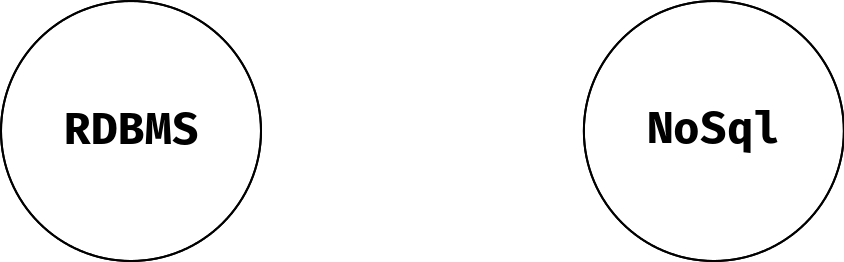
\includegraphics[width=0.8\textwidth,center]{rdbms_nosql_1.png}
    \end{figure}
\end{frame}

\begin{frame}[fragile]
    \frametitle{Философское введение}
    \vspace{-35pt}
    \begin{figure}
        
\includegraphics[width=0.8\textwidth,center]{rdbms_nosql_2.png}
    \end{figure}
\end{frame}

\begin{frame}[fragile]
    \frametitle{Философское введение}
    Почему это важно?
    Каков уровень поддержки хранения \\ слабо-структурированных данных в PostgreSQL?
\end{frame}

\begin{frame}
    \frametitle{Философское введение}
    \vspace{-35pt}
    \begin{figure}
        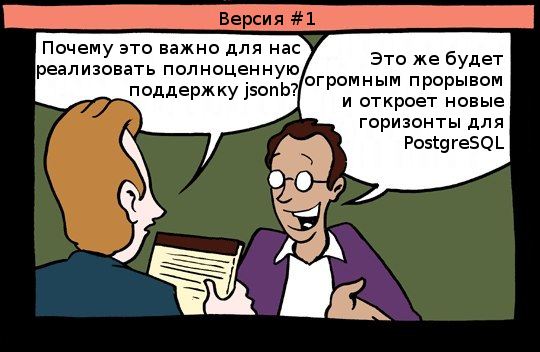
\includegraphics[width=0.8\textwidth,center]{first_option.png}
    \end{figure}
\end{frame}

\begin{frame}
    \frametitle{Философское введение}
    \vspace{-35pt}
    \begin{figure}
        
\includegraphics[width=0.8\textwidth,center]{second_option.png}
    \end{figure}
\end{frame}

\begin{frame}[fragile]
    \frametitle{Философское введение}
    \vspace{-35pt}
    \begin{figure}
        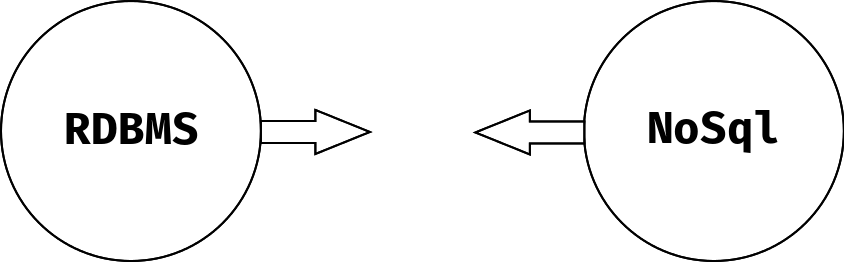
\includegraphics[width=0.8\textwidth,center]{rdbms_nosql_3.png}
    \end{figure}
\end{frame}
\note{
    Помимо PG и прочего упомянут про BI connector from MongoDB
}

\begin{frame}
    \frametitle{Философское введение}
    \vspace{-39pt}
    \begin{figure}
        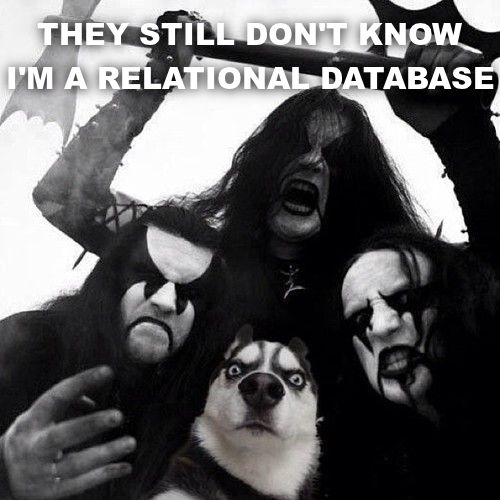
\includegraphics[width=0.55\textwidth,center]{black_metal_dog2.jpg}
    \end{figure}
\end{frame}

\section{Сравнение функционала}

\begin{frame}[fragile]
    \frametitle{Обзор по категориям}

    \begin{adjustbox}{max totalsize={1.1\textwidth}{2.0\textheight},center}
        \begin{tabular}{c | c | c | c | c | c | c | c | c | c | c}
            DB & Native & Select & Modify & Delete & Attributes & Indexing & Search & Convertion & Syntastic \\
            \hline
            PG & \check & \check & \check & \check & \check & \check & \question & \check & \question \\
            Mysql & \check & \check & \check & \check & \check & \question & \question & \fail & \question \\
            Oracle & \fail & \check & \fail & \fail & \fail & \fail & \question & \question & \question \\
            DB2 & \check & \fail & \fail & \fail & \fail & \fail & \fail & \question & \fail \\
            MSSql & \fail & \check & \fail & \fail & \fail & \fail & \question & \question & \fail \\
        \end{tabular}
    \end{adjustbox}
\end{frame}

\section{PostgreSQL}

\begin{frame}[fragile]
    \frametitle{PostgreSQL}
    \begin{itemize}[label={\MVRightarrow}]
        \item Hstore
        \item Json
        \item \alert{Jsonb + (jsonbx)}
    \end{itemize}

    PostgreSQL 9.5
\end{frame}
    
\begin{frame}[fragile]
    \frametitle{Многоликий Jsonb}

  \begin{itemize}
      \item<+->
          \begin{lstlisting}[
              basicstyle=\footnotesize\ttfamily,
              showstringspaces=false,
          ]
select '"string"'::jsonb;
         
          \end{lstlisting}

      \item<+->
          \begin{lstlisting}[
              basicstyle=\footnotesize\ttfamily,
              showstringspaces=false,
          ]
select '1'::jsonb;
         
          \end{lstlisting}

      \item<+->
          \begin{lstlisting}[
              basicstyle=\footnotesize\ttfamily,
              showstringspaces=false,
          ]
select 'true'::jsonb;
         
          \end{lstlisting}

      \item<+->
          \begin{lstlisting}[
              basicstyle=\footnotesize\ttfamily,
              showstringspaces=false,
          ]
select '[1, 2, 3]'::jsonb;
         
          \end{lstlisting}

      \item<+->
          \begin{lstlisting}[
              basicstyle=\footnotesize\ttfamily,
              showstringspaces=false,
          ]
select '["string", 1]'::jsonb;
         
          \end{lstlisting}

      \item<+->
          \begin{lstlisting}[
              basicstyle=\footnotesize\ttfamily,
              showstringspaces=false,
          ]
select '{"key": {"nested": "value"}}'::jsonb;
         
          \end{lstlisting}

  \end{itemize}

\end{frame}

\begin{frame}[fragile]
  \frametitle{Получение данных}

  \begin{itemize}
      \item
          \begin{lstlisting}[
              basicstyle=\footnotesize\ttfamily,
              showstringspaces=false,
          ]
select '{"key": "value"}'::jsonb ->> 'key';
         
          \end{lstlisting}

      \item
          \begin{lstlisting}[
              basicstyle=\footnotesize\ttfamily,
              showstringspaces=false,
          ]
select '["string", (*@\alert{1}@*)]'::jsonb -> -1;
         
          \end{lstlisting}

      \item
          \begin{lstlisting}[
              basicstyle=\footnotesize\ttfamily,
              showstringspaces=false,
          ]
select '{
    (*@\alert{"key"}@*): {(*@\alert{"nested\_key"}@*): "value"}
}'::jsonb #> '{key, nested_key}'
         
          \end{lstlisting}

  \end{itemize}

\end{frame}

\begin{frame}[fragile]
  \frametitle{Изменение данных}

  \begin{lstlisting}[
      basicstyle=\footnotesize\ttfamily,
      showstringspaces=false,
  ]
select jsonb_set(
    '{"n":null, "a":{"b": 2}}'::jsonb,
    '{n}',
    '[1,2,3]'
);

            jsonb_set                                 
-------------------------------------
{"a": {"b": 2}, "n": [1, 2, 3]}
 (1 row)
 
  \end{lstlisting}

\end{frame}

\begin{frame}[fragile]
  \frametitle{Удаление данных}

  \begin{lstlisting}[
      basicstyle=\footnotesize\ttfamily,
      showstringspaces=false,
  ]

select 
    '{"a": {"b": [1, 2, (*@\alert{3}@*)]}}'::jsonb
    #-
    '{a, b, -1}';
       ?column?       
----------------------
 {"a": {"b": [1, 2]}}
(1 row)

  \end{lstlisting}
\end{frame}

\begin{frame}[fragile]
  \frametitle{Аттрибуты}

\begin{lstlisting}[
  basicstyle=\footnotesize\ttfamily,
  showstringspaces=false,
]

select jsonb_object_keys(
    '{"key": "value"}'::jsonb
);

 jsonb_object_keys 
-------------------
 key
(1 row)
         
\end{lstlisting}

\end{frame}

\begin{frame}[fragile]
  \frametitle{Аттрибуты}

\begin{lstlisting}[
  basicstyle=\footnotesize\ttfamily,
  showstringspaces=false,
]

select jsonb_typeof('1'::jsonb);

 jsonb_typeof 
--------------
 number
(1 row)

\end{lstlisting}

\end{frame}

\begin{frame}[fragile]
  \frametitle{Индексирование}

  \begin{itemize}[label={\MVRightarrow}]
    \item GIN индекс для @> <@ ?
    \item jsonb\_path\_ops
    \item jsquery: jsonb\_path\_value, jsonb\_path\_key
  \end{itemize}

\end{frame}

\begin{frame}[fragile]
  \frametitle{Поиск}

  \begin{itemize}[label={\MVRightarrow}]
    \item Содержит ли jsonb объект указанных ключ?
    \item jsquery
  \end{itemize}

\end{frame}

\begin{frame}[fragile]
  \frametitle{Конвертирование}

  \vspace{-20pt}
\begin{lstlisting}[]

select * from test_agg;
 id |   data   
----+----------
  1 | value1
  2 | value2
(2 rows)
         
\end{lstlisting}

\begin{lstlisting}[]

select jsonb_pretty(jsonb_agg(test_agg)) from test_agg;
         jsonb_pretty         
------------------------------
 [                           +
     {                       +
         "id": 1,            +
         "data": "value1"    +
     },                      +
     {                       +
         "id": 2,            +
         "data": "value2"    +
     }                       +
 ]
(1 row)

\end{lstlisting}

\end{frame}

\begin{frame}[fragile]
  \frametitle{Конвертирование}

\begin{lstlisting}[
  basicstyle=\footnotesize\ttfamily,
  showstringspaces=false,
]

select array_to_json(
    ARRAY [
        jsonb '{"a":1}',
        jsonb '{"b":[2,3]}'
    ]
);
      array_to_json       
--------------------------
 [{"a": 1},{"b": [2, 3]}]
(1 row)

\end{lstlisting}

\end{frame}

\begin{frame}[fragile]
  \frametitle{Синтаксис}

\begin{lstlisting}[
  basicstyle=\footnotesize\ttfamily,
  showstringspaces=false,
]
update some_table set jsonb_data =
    jsonb_set(jsonb_data, '{a, a1, a2}', '42');
\end{lstlisting}

vs

\begin{lstlisting}[
  basicstyle=\footnotesize\ttfamily,
  showstringspaces=false,
]

update some_table
    set jsonb_data['a']['a1']['a2'] = 42;

\end{lstlisting}

\end{frame}

\section{MySql}

\begin{frame}[fragile]
    \frametitle{MySql}

    MySql 5.7.7, тип данных JSON
\end{frame}
    
\begin{frame}[fragile]
    \frametitle{Возможные виды}

  \begin{itemize}
      \item<+->
          \begin{lstlisting}[
              basicstyle=\footnotesize\ttfamily,
              showstringspaces=false,
          ]
select cast('"string"' as json);
         
          \end{lstlisting}

      \item<+->
          \begin{lstlisting}[
              basicstyle=\footnotesize\ttfamily,
              showstringspaces=false,
          ]
select cast('["string", 1]' as json);
         
          \end{lstlisting}

      \item<+->
          \begin{lstlisting}[
              basicstyle=\footnotesize\ttfamily,
              showstringspaces=false,
          ]
select cast('{"key": {"nested": "value"}}' as json);
         
          \end{lstlisting}

  \end{itemize}

\end{frame}

\begin{frame}[fragile]
  \frametitle{Получение данных}

  \begin{itemize}
      \item
          \begin{lstlisting}[
              basicstyle=\footnotesize\ttfamily,
              showstringspaces=false,
          ]
select json_extract('{"key": "value"}', '$.*');
         
          \end{lstlisting}

      \item
          \begin{lstlisting}[
              basicstyle=\footnotesize\ttfamily,
              showstringspaces=false,
          ]
select cast('{"key": "value"}' as json) -> 'key';
         
          \end{lstlisting}

  \end{itemize}

\end{frame}

\begin{frame}[fragile]
  \frametitle{Изменение данных}

  \begin{lstlisting}[
      basicstyle=\footnotesize\ttfamily,
      showstringspaces=false,
  ]
select json_set(
    '{"n":null, "a":{"b": 2}}',
    '$.n',
    '[1,2,3]',
    '$.a',
    1
);

--------------------------
{"a": 1, "n": "[1,2,3]"}
1 row in set (0.01 sec)
 
  \end{lstlisting}

\end{frame}
\note{
    Упомянуть про то, что пока в pg нет jsonb\_insert
    для массивов
}

\begin{frame}[fragile]
  \frametitle{Удаление данных}

  \begin{lstlisting}[
      basicstyle=\footnotesize\ttfamily,
      showstringspaces=false,
  ]

select json_remove(
    '{"a": {"b": [1, 2, 3]}}',
    '$.a.b[2]'
)

----------------------
{"a": {"b": [1, 2]}}
1 row in set (0.01 sec)

  \end{lstlisting}
\end{frame}

\begin{frame}[fragile]
  \frametitle{Аттрибуты}

\begin{lstlisting}[
  basicstyle=\footnotesize\ttfamily,
  showstringspaces=false,
]

select json_type('1');

--------------
INTEGER
1 row in set (0.01 sec)

\end{lstlisting}

\end{frame}

\begin{frame}[fragile]
  \frametitle{Аттрибуты}
  Нет методов для получения ключей, значений и проч.\\
  Есть методы для получения длинны или глубины json.

\end{frame}

\begin{frame}[fragile]
  \frametitle{Индексирование}
  Тип json на прямую не индексируется, в качестве workaround\\
  предлагается создавать generated поля с json\_extract.
\end{frame}

\begin{frame}[fragile]
  \frametitle{Поиск}

  \vspace{-20pt}
  \begin{itemize}[label={\MVRightarrow}]
    \item Поиск в пути \$, *
    \item Поиск по значению json\_search
  \end{itemize}

\begin{lstlisting}[
  basicstyle=\footnotesize\ttfamily,
  showstringspaces=false,
]

select json_search(
    '{"a": "test", "b": [1, 2, "test2"]}',
    'all', 'test%'
);

--------------
["$.a", "$.b[2]"]
1 row in set (0.00 sec)

\end{lstlisting}


\end{frame}

\section{Oracle}

\begin{frame}[fragile]
    \frametitle{Oracle}

    Oracle 12.1.0.2, тип данных JSON\\
    Требует \textbf{WITH UNIQUE KEYS}
\end{frame}

\begin{frame}[fragile]
  \frametitle{Получение данных}

  \begin{itemize}
      \item
          \begin{lstlisting}[
              basicstyle=\footnotesize\ttfamily,
              showstringspaces=false,
          ]
SELECT json.document.Nested.key FROM json_data json;
         
          \end{lstlisting}

      \item
          \begin{lstlisting}[
              basicstyle=\footnotesize\ttfamily,
              showstringspaces=false,
          ]
SELECT json_value(document, '$.Number' RETURNING NUMBER) FROM json_document;

         
          \end{lstlisting}

  \end{itemize}

\end{frame}

\begin{frame}[fragile]
    \frametitle{Тест}

    \begin{adjustbox}{max totalsize={1.0\textwidth}{.7\textheight},center}
        \begin{tikzpicture}[node distance = 2.5cm, auto]
            \node[block] (hstore){
                Hstore
            };

            \node[block, below of=hstore] (nested_hstore){
                Nested Hstore
            };

            \node[block, below of=nested_hstore] (jsonb){
                Jsonb
            };

            \path[line] (hstore) -- (nested_hstore);
            \path[line, dashed] (nested_hstore) -- (jsonb);

        \end{tikzpicture}
    \end{adjustbox}
\end{frame}
\note{
  Hstore is a key-value binary storage.
  Doesn't support tree-like nested structures,
  but there is a nested version of hstore.

  Binary JSON storage. JSONB was introduced in PostgreSQL 9.4 and
  supports fast lookups and simple expression search queries using
  Generalized Inverted Indexes (GIN). It supposed to be document-oriented
  and was designed for the schema-less data.
}

\begin{frame}[fragile]
    \frametitle{Many faces of jsonb}

  \begin{itemize}
      \item<+->
          \begin{lstlisting}[
              basicstyle=\footnotesize\ttfamily,
              showstringspaces=false,
          ]
select '"string"'::jsonb;
         
          \end{lstlisting}

      \item<+->
          \begin{lstlisting}[
              basicstyle=\footnotesize\ttfamily,
              showstringspaces=false,
          ]
select '1'::jsonb;
         
          \end{lstlisting}

      \item<+->
          \begin{lstlisting}[
              basicstyle=\footnotesize\ttfamily,
              showstringspaces=false,
          ]
select 'true'::jsonb;
         
          \end{lstlisting}

      \item<+->
          \begin{lstlisting}[
              basicstyle=\footnotesize\ttfamily,
              showstringspaces=false,
          ]
select '[1, 2, 3]'::jsonb;
         
          \end{lstlisting}

      \item<+->
          \begin{lstlisting}[
              basicstyle=\footnotesize\ttfamily,
              showstringspaces=false,
          ]
select '["string", 1]'::jsonb;
         
          \end{lstlisting}

      \item<+->
          \begin{lstlisting}[
              basicstyle=\footnotesize\ttfamily,
              showstringspaces=false,
          ]
select '{"key": {"nested": "value"}}'::jsonb;
         
          \end{lstlisting}

  \end{itemize}

\end{frame}
\note{
 * When a naked
 * scalar value needs to be stored as a Jsonb value, what we actually store is
 * an array with one element, with the flags in the array's header field set
 * to JB\_FSCALAR | JB\_FARRAY.

 Note about deduplication and space trimming
}

\begin{frame}[fragile]
  \frametitle{Lack of some functionality}
  Тест тест

  \begin{itemize}
      \item[\MVRightarrow] Get an element at arbitrary path ( \#> )
      \item[\MVRightarrow] Delete an element at arbitrary path  ( ? )
      \item[\MVRightarrow] Update an element at arbitrary path ( ? )
      \item[\MVRightarrow] Add a new element to arbitrary path ( ? )
  \end{itemize}

\end{frame}

\begin{frame}[fragile]
  \frametitle{jsonbx}

  Pgxn extension for PostgreSQL 9.4, which contains implementation of
  some missing functionality. It based on nested version of hstore
  and provided this functions for the corresponding patch for 9.5

\end{frame}

\section{Get data}

\begin{frame}[fragile]
  \frametitle{By key}

  \begin{itemize}
      \item
          \begin{lstlisting}[
              basicstyle=\footnotesize\ttfamily,
              showstringspaces=false,
          ]
select '{"key": "value"}'::jsonb -> 'key';
         
          \end{lstlisting}

      \item
          \begin{lstlisting}[
              basicstyle=\footnotesize\ttfamily,
              showstringspaces=false,
          ]
select '{"key": "value"}'::jsonb ->> 'key';
         
          \end{lstlisting}

  \end{itemize}

\end{frame}

\begin{frame}[fragile]
  \frametitle{By index}

  \begin{itemize}
      \item
          \begin{lstlisting}[
              basicstyle=\footnotesize\ttfamily,
              showstringspaces=false,
          ]
select '[(*@\alert{"string"}@*), 1]'::jsonb -> 0;
         
          \end{lstlisting}

      \item
          \begin{lstlisting}[
              basicstyle=\footnotesize\ttfamily,
              showstringspaces=false,
          ]
select '["string", (*@\alert{1}@*)]'::jsonb -> -1;
         
          \end{lstlisting}

  \end{itemize}

\end{frame}

\begin{frame}[fragile]
  \frametitle{By path}

  \begin{itemize}
      \item[\MVRightarrow] Point out an element inside a jsonb field
      \item[\MVRightarrow] Technically, it's just an array of items
      \item[\MVRightarrow] Each element is an index (include negative values) or a key
      \item
          \begin{lstlisting}[
              basicstyle=\footnotesize\ttfamily,
              showstringspaces=false,
          ]
'{first_key, second_key, 1, -1}'
         
          \end{lstlisting}

  \end{itemize}

\end{frame}

\begin{frame}[fragile]
  \frametitle{By path}

  \begin{itemize}
      \item
          \begin{lstlisting}[
              basicstyle=\footnotesize\ttfamily,
              showstringspaces=false,
          ]
select '{
    (*@\alert{"key"}@*): {(*@\alert{"nested\_key"}@*): "value"}
}'::jsonb #> '{key, nested_key}'
         
          \end{lstlisting}

      \item
          \begin{lstlisting}[
              basicstyle=\footnotesize\ttfamily,
              showstringspaces=false,
          ]

select '{
    (*@\alert{"key"}@*): [1, 2, (*@\alert{"string"}@*)]
}'::jsonb #> '{key, -1}'
         
          \end{lstlisting}

  \end{itemize}

\end{frame}

\section{Know your data}

\begin{frame}[fragile]
  \frametitle{Contains or contained?}

  \begin{itemize}
      \item
          \begin{lstlisting}[
              basicstyle=\footnotesize\ttfamily,
              showstringspaces=false,
          ]

select
    '{"a": 1, "b": 1}'::jsonb
    @>
    '{"a": 1}'::jsonb
         
          \end{lstlisting}

      \item
          \begin{lstlisting}[
              basicstyle=\footnotesize\ttfamily,
              showstringspaces=false,
          ]

select '[1]'::jsonb <@ '[1, 2]'::jsonb
         
          \end{lstlisting}


  \end{itemize}

\end{frame}

\begin{frame}[fragile]
  \frametitle{Equality}

    \begin{lstlisting}[
      basicstyle=\footnotesize\ttfamily,
      showstringspaces=false,
    ]

select
    '{"key":"value"}'::jsonb
    <>
    '{"key":"another_value"}'::jsonb;

    \end{lstlisting}

    \begin{lstlisting}[
      basicstyle=\footnotesize\ttfamily,
      showstringspaces=false,
    ]

select
    '{"key":"value"}'::jsonb
    =
    '{"key":"another_value"}'::jsonb;

    \end{lstlisting}

\end{frame}

\begin{frame}[fragile]
  \frametitle{jsonb\_pretty}

  \begin{lstlisting}[]
select jsonb_pretty('{"a":"test","b":[1,2,3],"c":"test3","d":{"dd":"test4","dd2":{"ddd":"test5"}}}'::jsonb);

        jsonb_pretty        
----------------------------
 {                         +
     "a": "test",          +
     "b": [                +
         1,                +
         2,                +
         3                 +
     ],                    +
     "c": "test3",         +
     "d": {                +
         "dd": "test4",    +
         "dd2": {          +
             "ddd": "test5"+
         }                 +
     }                     +
 }
(1 row)
  \end{lstlisting}

\end{frame}

\begin{frame}[fragile]
  \frametitle{Aggregation}

  \vspace{-20pt}
\begin{lstlisting}[]

select * from test_agg;
 id |   data   
----+----------
  1 | value1
  2 | value2
(2 rows)
         
\end{lstlisting}

\begin{lstlisting}[]

select jsonb_pretty(jsonb_agg(test_agg)) from test_agg;
         jsonb_pretty         
------------------------------
 [                           +
     {                       +
         "id": 1,            +
         "data": "value1"    +
     },                      +
     {                       +
         "id": 2,            +
         "data": "value2"    +
     }                       +
 ]
(1 row)

\end{lstlisting}

\end{frame}

\begin{frame}[fragile]
  \frametitle{Get keys}

\begin{lstlisting}[
  basicstyle=\footnotesize\ttfamily,
  showstringspaces=false,
]

select jsonb_object_keys(
    '{"key": "value"}'::jsonb
);

 jsonb_object_keys 
-------------------
 key
(1 row)
         
\end{lstlisting}

\end{frame}

\section{Build \& transform}

\begin{frame}[fragile]
  \frametitle{Build}

\begin{lstlisting}[
  basicstyle=\footnotesize\ttfamily,
  showstringspaces=false,
]

select jsonb_build_object('key', 'value');
 jsonb_build_object 
--------------------
 {"key": "value"}
(1 row)

\end{lstlisting}

\begin{lstlisting}[
  basicstyle=\footnotesize\ttfamily,
  showstringspaces=false,
]

select jsonb_object('{key, value}');
   jsonb_object   
------------------
 {"key": "value"}
(1 row)

\end{lstlisting}

\end{frame}

\begin{frame}[fragile]
  \frametitle{Build}

\begin{lstlisting}[
  basicstyle=\footnotesize\ttfamily,
  showstringspaces=false,
]

select jsonb_build_array('string', 1);                                                                                                                  
 jsonb_build_array 
-------------------
 ["string", 1]
(1 row)

\end{lstlisting}

\end{frame}

\begin{frame}[fragile]
  \frametitle{Populate record}

\begin{lstlisting}[
  basicstyle=\footnotesize\ttfamily,
  showstringspaces=false,
]

create type data_type as (key text, value text);

select * from jsonb_populate_record(
    null::data_type,
    '{"key": "some_key", "value": "some_data"}'
);

   key    |   value   
----------+-----------
 some_key | some_data
(1 row)

\end{lstlisting}

\end{frame}


\section{Manipulation with jsonb}

\begin{frame}[fragile]
  \frametitle{jsonb\_set: replace value}

  \begin{lstlisting}[
      basicstyle=\footnotesize\ttfamily,
      showstringspaces=false,
  ]
select jsonb_set(
    '{"n":null, "a":{"b": 2}}'::jsonb,
    '{n}',
    '[1,2,3]'
);

            jsonb_set                                 
-------------------------------------
{"a": {"b": 2}, "n": [1, 2, 3]}
 (1 row)
 
  \end{lstlisting}

\end{frame}

\begin{frame}[fragile]
  \frametitle{jsonb\_set: create mode by default}

  \begin{lstlisting}[
      basicstyle=\footnotesize\ttfamily,
      showstringspaces=false,
  ]
select jsonb_set(
    '{"a":{"b": 2}}'::jsonb,
    '{c}',
    '[1,2,3]'
);

            jsonb_set                                 
-------------------------------------
{"a": {"b": 2}, (*@\alert{"c": [1, 2, 3]}@*)}
 (1 row)
 
  \end{lstlisting}

\end{frame}

\begin{frame}[fragile]
  \frametitle{jsonb\_set: turn off the create mode}

  \begin{lstlisting}[
      basicstyle=\footnotesize\ttfamily,
      showstringspaces=false,
  ]
select jsonb_set(
    '{"a":{"b": 2}}'::jsonb,
    '{c}',
    '[1,2,3]',
    (*@\alert{false}@*)
);

    jsonb_set    
-----------------
 {"a": {"b": 2}}
(1 row)
 
  \end{lstlisting}

\end{frame}

\begin{frame}[fragile]
  \frametitle{jsonb\_delete: by key}

  \begin{lstlisting}[
      basicstyle=\footnotesize\ttfamily,
      showstringspaces=false,
  ]
select '{"a":1 , "b":2, "c":3}'::jsonb - 'a';

     ?column?     
------------------
 {"b": 2, "c": 3}
(1 row)

  \end{lstlisting}
\end{frame}
\note{jsonb\_delete(jsonb, text) allow to delete only top level key from object}

\begin{frame}[fragile]
  \frametitle{jsonb\_delete: by index}

  \begin{lstlisting}[
      basicstyle=\footnotesize\ttfamily,
      showstringspaces=false,
  ]
select '["a", "b", "c"]'::jsonb - 2;

  ?column?  
------------
 ["a", "b"]
(1 row)

  \end{lstlisting}
\end{frame}

\begin{frame}[fragile]
  \frametitle{jsonb\_delete: by path}

  \begin{lstlisting}[
      basicstyle=\footnotesize\ttfamily,
      showstringspaces=false,
  ]

select 
    '{"a": {"b": [1, 2, (*@\alert{3}@*)]}}'::jsonb
    #-
    '{a, b, -1}';
       ?column?       
----------------------
 {"a": {"b": [1, 2]}}
(1 row)

  \end{lstlisting}
\end{frame}

\begin{frame}[fragile]
\frametitle{jsonb\_concat ("shallow concatenation")}

  \begin{lstlisting}[
      basicstyle=\footnotesize\ttfamily,
      showstringspaces=false,
  ]
select 
    '{"a": 1, "b": [2, 3]}'::jsonb
    ||
    '{"a": 4, "c": [5, 6]}'::jsonb

              ?column?              
------------------------------------
 {"a": 4, "b": [2, 3], "c": [5, 6]}
(1 row)

  \end{lstlisting}
\end{frame}
\note{
    This operator is questionable, and I'm not sure how it will be in 9.5,
    but I think it will be present in this form in jsonbx extension
}

\begin{frame}[fragile]
\frametitle{jsonb\_concat ("shallow concatenation")}

  \begin{lstlisting}[
      basicstyle=\footnotesize\ttfamily,
      showstringspaces=false,
  ]
select 
    '{"key": {"nested_key": "value"}}'::jsonb
    ||
    '{"key": {"another_key": "another_value"}}'::jsonb

                 ?column?                  
-------------------------------------------
 {"key": {"another_key": "another_value"}}
(1 row)

  \end{lstlisting}
\end{frame}

\begin{frame}[fragile]
\frametitle{jsonb\_concat ("shallow concatenation")}
    Array will consume an object
  \begin{lstlisting}[
      basicstyle=\footnotesize\ttfamily,
      showstringspaces=false,
  ]
select 
    '{"key": "value"}'::jsonb
    ||
    '[1, 2, 3]'::jsonb 

          ?column?           
-----------------------------
 [{"key": "value"}, 1, 2, 3]
(1 row)

  \end{lstlisting}
\end{frame}

\begin{frame}[fragile]
\frametitle{jsonb\_concat ("shallow concatenation")}
    Scalars are acting like arrays
  \begin{lstlisting}[
      basicstyle=\footnotesize\ttfamily,
      showstringspaces=false,
  ]
select '"b"'::jsonb || '"a"'::jsonb

  ?column?  
------------
 ["b", "a"]

  \end{lstlisting}
\end{frame}

\section{Performance}

\section{Comparison}

\section{Plans for the future}

\begin{frame}[fragile]
  \frametitle{Array-style subscripting}

  \begin{itemize}
      \item
      \begin{lstlisting}[
          basicstyle=\footnotesize\ttfamily,
          showstringspaces=false,
      ]
update some_table
    set jsonb_data['a']['a1']['a2'] = 42;

      \end{lstlisting}

      \item
      \begin{lstlisting}[
          basicstyle=\footnotesize\ttfamily,
          showstringspaces=false,
      ]
select jsonb_data['a']['a1']['a2']
    from some_table;

      \end{lstlisting}
  \end{itemize}

\end{frame}

\begin{frame}[fragile]
  \frametitle{Jsonb pointer \& patch}

  \begin{itemize}
      \item[\MVRightarrow] Json pointer [\href{http://tools.ietf.org/html/rfc6901}{rfc6901}]
      \item[\MVRightarrow] Json patch [\href{http://tools.ietf.org/html/rfc6902}{rfc6901}]
  \end{itemize}

\end{frame}

\begin{frame}[fragile]
  \frametitle{New functions and improvements}

  There are still missing functionality and improvements, that can be useful for JSONB.
  Some of them will be implented as parts of jsonbx extension (for 9.5), and will be proposed for 9.6
\end{frame}

\begin{frame}[fragile]
  \frametitle{jsonb\_delete}

  \begin{lstlisting}[
      basicstyle=\footnotesize\ttfamily,
      showstringspaces=false,
  ]
select jsonb_delete_jsonb(
    '{"a": 1, "b": {"c": 2}, (*@\alert{"f": [4, 5]}@*)}'::jsonb,
    '{"a": 4, (*@\alert{"f": [4, 5]}@*), "c": 2}'::jsonb
);

      jsonb_delete
----------------------------
  {"a": 1, "b": {"c": 2}}
(1 row)

  \end{lstlisting}

\end{frame}

\begin{frame}[fragile]
  \frametitle{jsonb\_intersection}

  \begin{lstlisting}[
      basicstyle=\footnotesize\ttfamily,
      showstringspaces=false,
  ]
select jsonb_intersection(
    '{(*@\alert{"a":2}@*), "d": {"f": 3}, (*@\alert{"g":[4, 5]}@*)}'::jsonb,
    '{(*@\alert{"a":2}@*), "f": 3, (*@\alert{"g":[4, 5]}@*)}'::jsonb
);

   jsonb_intersection
--------------------------
  {"a": 2, "g": [4, 5]}
(1 row)

  \end{lstlisting}

\end{frame}

\begin{frame}[fragile]
  \frametitle{jsonb\_deep\_merge}

  \begin{lstlisting}[
      basicstyle=\footnotesize\ttfamily,
      showstringspaces=false,
  ]
select jsonb_deep_merge(
    '{"a": (*@\alert{\{"b":1\}}@*)}'::jsonb,
    '{"a": (*@\alert{\{"c":2\}}@*)}'::jsonb
);

     jsonb_deep_merge            
-------------------------------
   {"a": (*@\alert{\{"b":1, "c":2\}}@*)}
(1 row)

  \end{lstlisting}

\end{frame}
\note{
    Form of this function is questionable,
    but I think it will be present in this form in jsonbx extension
}

\section{Finish}

\begin{frame}{Contacts}
    \begin{itemize}[label={}]
        \item \href{https://github.com/erthalion/jsonbx}{\github\ github.com/erthalion/jsonbx}
        \item \href{http://twitter.com/erthalion}{\twitter\ @erthalion}
        \item \email\ 9erthalion6 at gmail dot com
    \end{itemize}
\end{frame}

\plain{Questions?}

\end{document}
